%!TEX root=../paper.tex

This section presents the design of ISE focusing on accelerating the operation of the ChaCha cipher's block function. 
The ISE-assisted acceleration for the ChaCha block function is fairly challenging especially for the scalar-register-based ISEs because 
a) The block function was designed to be very efficient on software without dedicated hardware support. 
b) The function computes on 32-bit state elements and two consecutive operations involve at least 3 different state elements. 
The latter poses difficulties for the acceleration using the scalar-register-based ISEs on 32-bit RISC-V architecture without the capable of having more than 2 source operands.
Certainly, vector instructions are possible approaches to accelerating ChaCha. 
But in this paper, we focused on the scalar-register-based ISE approaches on RISC-V architecture instead. 
This provides a lower area overhead solution compared to vectorisation alternatives. 

Our ISE designs obey the wider RISC-V design principles. 
This means the ISE designs should support simple building-block operations, and their instruction encodings must be at most 2 source registers and 1 destination register. 
By following that the proposed ISEs can be straightforwardly integrated into different existing RISC-V implementations with negligible modification.
To ensure low area and latency overheads, the proposed ISEs follow further requirements: 
a) The ISE must store operands and results in the RISC-V general-purpose scalar register file. 
b) The ISE must not introduce special-purpose architectural states, nor rely on special-purpose micro-architectural state (e.g., registers, caches, or scratch-pad memory).
c) The operation of ISE should be implemented to execute in one clock cycle in its hardware module and must guaranteeing constant-time execution that can  inherently prevent certain attack vectors based on execution latency (see~\cite[Section 4]{GYC:18}).

Overall, the proposed ISEs intentionally target performing ChaCha stream cipher on low(er)-end, resource-constrained devices such as embedded IoT edge computing that don't support a vector engine. The focus can be viewed as reasonable because existing work on adding cryptographic support to the standard vector extension \cite{riscv:ext:vector:draft} already caters for high(er)-end alternatives. 

\subsection{ISE Design for 32-bit architecture}

The challenge to accelerate the ChaCha block function using 32-bit ISEs is to fetching sufficient state elements, i.e., operands for the ISE operations.
We consider potential options for 32 bit-architectures, namely, accessing register pairs and having additional registers in the ISE.
Both options can help to fetch additional state elements for the ChaCha round accelerator. 
However, the former may, apart from violating the design constraints of RISCV, 
increase the complexity of decoder and register files, and 
induce increased size of pipeline stages' registers to accommodate the additional operands.
The latter introduces additional states in the ISE that may cause the dirty state issues in context switching scenarios (e.g., interrupt handling, multitasking).
that requires additional flushing and/or synchronisation mechanisms leading to significant performance reduction.
Because of the aforementioned reasons, these two options are not well suite for a lightweight solution to accelerate the ChaCha round function.

Another possible alternative is straightforwardly combining rotation and arithmetic/logical operations. 
This alternative can obviously reduce the number of instruction count, hence improve the performance, for the ChaCha round function.
However, the gains are fairly limited. 
For example, a ISE combining 32-bit XOR and 32-bit rotation can reduce the instruction count of the ChaCha quarter round function from 
12 to 8. 
That results in the maximum instruction count reduction achieved by using the ISE to about 66.67\% of the instruction count of the implementation without ISEs support.

\subsection{ISE Design for 64-bit architecture}
The 64-bit architecture allows each instruction to pack more ChaCha state elements (e.g. 2-source-operands instructions can pack 4 ChaCha state elements) compared to 32-bit architectures. 
This enables the possibility of efficient accelerations.
We arrive at four ISE variants, the design of which is split into intuitive descriptions in the following subsections. 

\subsubsection{Variant 1 ($V_1$)}
$V_1$ is based on a performance-oriented approach which aims at executing the ChaCha quarter round with a minimal number of instructions.
Due to the 1-destination-register constraint, the ChaCha quarter round can be executed at least two ISEs to compute 4 state elements of the quarter round.
Therefore, we propose two ISEs as follows:

\begin{itemize}

\INST{chacha20.v1.ad    rd, rs1, rs2}{
  uint32\xspace $a,b,c,d, ia, ib, ic,id, na,nd$; \;
  $a \ASN \GPR[*][{\VERB[ASM]{rs1}}] \RSH 32; d \ASN \GPR[*][{\VERB[ASM]{rs1}}];$ \;
  $b \ASN \GPR[*][{\VERB[ASM]{rs2}}] \RSH 32; c \ASN \GPR[*][{\VERB[ASM]{rs2}}];$ \;
  $ia \ASN a + b; id \ASN (ia \XOR  d) \LRT 16;$ \;
  $ic \ASN c +id; ib \ASN (ic \XOR  b) \LRT12;$ \;
  $na \ASN ia+ib; $ \;
  $nd \ASN (id \XOR na) \LRT 8;$ \;
  $\GPR[*][{\VERB[ASM]{rd}}] \ASN (na \LSH 32) \IOR nd;$ \;
}

\INST{chacha20.v1.bc    rd, rs1, rs2}{
  uint32\xspace $a,b,c,d, ib, ic,id, na,nd$; \;
  $a \ASN \GPR[*][{\VERB[ASM]{rs1}}] \RSH 32; d \ASN \GPR[*][{\VERB[ASM]{rs1}}];$ \;
  $b \ASN \GPR[*][{\VERB[ASM]{rs2}}] \RSH 32; c \ASN \GPR[*][{\VERB[ASM]{rs2}}];$ \;
  $id \ASN (d \LRT 24) \XOR a; ic \ASN c \XOR id; ib \ASN (b \XOR ic) \LRT 12;$ \;
  $nc \ASN ic+ d; $ \;
  $nb \ASN (ib \XOR nc) \LRT 7;$ \;
  $\GPR[*][{\VERB[ASM]{rd}}] \ASN (nb \LSH 32) \IOR nc;$ \;
}
\end{itemize}

Each instruction takes two 64-bit-register operands \VERB[ASM]{rs1} and \VERB[ASM]{rs2}, each of which packs two 32-bit input elements of the quarter-round function. \VERB[ASM]{rs1} (resp. \VERB[ASM]{rs2}) contains two inputs $iA$ and $iD$ (resp. $iB$ and $iC$). \VERB{chacha20.v1.ad} (resp. \VERB{chacha20.v1.bc}) computes the outputs $oA$ and $oD$ (resp. $oB$ and $oC$) packed in its destination register \VERB[ASM]{rd}. 
This ISE variant can be used to implement the quarter-round function as in Algorithm~\ref{alg::qr::v1}.

\begin{algorithm}
\KwData  {64-bit values $X=\{iA \CONS iD \}$ and $Y=\{iB \CONS iC \}$.
}
\KwResult{64-bit values $R0$, $R1$ such that $R0=\{oA \CONS oD \}$ and $R1=\{oB \CONS oC \}$).
}
\BlankLine
\KwFn{$\ALG{QuarterRound}( X, Y )$}{
  \VERB[ASM]{chacha20.v1.ad} R0, X, Y \;
  \VERB[ASM]{chacha20.v1.bc} R1, R0, Y \;
  $\KwRet{\TUPLE{ R0, R1 }}$ \;
}
\caption{ChaCha Quarter Round in the Variant 1.}
\label{alg::qr::v1}
\end{algorithm}


\subsubsection{Variant 2 ($V_2$)}
As focusing on performance, the implementation of $V_1$ can lead to an un-optimal area overhead of four 32-bit \VERB{Xors} and three 32-bit \VERB{Additions}. $V_2$ present a trade-off approach to reduce area overhead by using 3 instructions. 
One ISE computes two intermediate values in the ChaCha quarter round function from the input state elements.
The other two ISEs calculates the output elements from the intermediate values and the input elements.
These ISEs are able to share their computational hardware (e.g. adder). By doing so, the $V_2$ reduces the required number of 32-bit additions from three to two compared to $V_1$. The ISEs of $V_2$ are described as follows:

\begin{itemize}

\INST{chacha20.v2.bd    rd, rs1, rs2}{
  uint32\xspace $a,b,c,d, nb,nd$; \;
  $a \ASN \GPR[*][{\VERB[ASM]{rs1}}] \RSH 32; d \ASN \GPR[*][{\VERB[ASM]{rs1}}];$ \;
  $b \ASN \GPR[*][{\VERB[ASM]{rs2}}] \RSH 32; c \ASN \GPR[*][{\VERB[ASM]{rs2}}];$ \;
  $nd \ASN ((a + b) \XOR d) \LRT 16;$ \;
  $nb \ASN ((c +nd) \XOR b) \LRT 12;$ \;
  $\GPR[*][{\VERB[ASM]{rd}}] \ASN (nb \LSH 32) \IOR nd;$ \;
}

\INST{chacha20.v2.ad    rd, rs1, rs2}{
  uint32\xspace $a,b',d',d, nb,nd$; \;
  $a  \ASN \GPR[*][{\VERB[ASM]{rs1}}] \RSH 32; d  \ASN \GPR[*][{\VERB[ASM]{rs1}}];$ \;
  $b' \ASN \GPR[*][{\VERB[ASM]{rs2}}] \RSH 32; d' \ASN \GPR[*][{\VERB[ASM]{rs2}}];$ \;
  $na \ASN b' + (d \XOR (d' \LRT 16));$ \; 
  $nd \ASN (na \XOR d') \LRT 8;$ \;
  $\GPR[*][{\VERB[ASM]{rd}}] \ASN (na \LSH 32) \IOR nd;$ \;
}

\INST{chacha20.v2.bc    rd, rs1, rs2}{
  uint32\xspace $a,b,c,d, t, na,nd$; \;
  $a  \ASN \GPR[*][{\VERB[ASM]{rs1}}] \RSH 32; d \ASN \GPR[*][{\VERB[ASM]{rs1}}];$ \;
  $b  \ASN \GPR[*][{\VERB[ASM]{rs2}}] \RSH 32; c \ASN \GPR[*][{\VERB[ASM]{rs2}}];$ \;
  $t  \ASN c + (d \LRT 24) \XOR a;$ \;
  $nc \ASN t + d;$ \;
  $nb \ASN (nc \XOR ((b \XOR t) \LRT 12)) \LRT 7;$ \;
  $\GPR[*][{\VERB[ASM]{rd}}] \ASN (nb \LSH 32) \IOR nc;$ \;
}
\end{itemize}

\VERB[ASM]{chacha20.v2.bd} computes the intermediate values packed in its destination resister \VERB[ASM]{rd} from 4 input elements $iA$, $iD$ (packed in \VERB[ASM]{rs1}), $iB$ and $iC$ (packed in \VERB[ASM]{rs2}).  \VERB{chacha20.v2.ad} (resp. \VERB{chacha20.v2.bc}) computes the outputs $oA$ and $oD$ (resp. $oB$ and $oC$) packed in its destination register \VERB[ASM]{rd} that is similar to the packing scheme in $V_1$. 
The quarter-round function can be implemented with 3 instructions as in Algorithm~\ref{alg::qr::v2}.
\begin{algorithm}
\KwData  {64-bit values $X=\{iA \CONS iD \}$ and $Y=\{iB \CONS iC \}$.
}
\KwResult{64-bit values $R0$, $R1$ such that $R0=\{oA \CONS oD \}$ and $R1=\{oB \CONS oC \}$).
}
\BlankLine
\KwFn{$\ALG{QuarterRound}( X, Y )$}{
  \VERB[ASM]{chacha20.v2.bd} T, X, Y  \;
  \VERB[ASM]{chacha20.v2.ad} R0, X, T \;
  \VERB[ASM]{chacha20.v2.bc} R1, R0, Y  \;
  $\KwRet{\TUPLE{ R0, R1 }}$ \;
}
\caption{ChaCha Quarter Round in the Variant 2.}
\label{alg::qr::v2}
\end{algorithm}

\subsubsection{Variant 3 ($V_3$)}
$V_3$ introduces an area-efficiency-oriented approach which aims at favouring hardware re-usage between ISEs to reduce overall area overhead. 
The approach is based on observing that the quarter round function can be split into two almost identical "top" and "bottom" halves. 
Moreover, each half consists of almost identical operation sequence including addition, xor, and rotation.
The only difference between these operation sequences is the left rotation amounts. 
So, we investigate four instructions to compute an entire quarter round as follows:

\begin{itemize}

\INST{chacha20.v3.ad0    rd, rs1, rs2}{
  uint32\xspace $a,b,d na,nd$; \;
  $a \ASN \GPR[*][{\VERB[ASM]{rs1}}] \RSH 32; d \ASN \GPR[*][{\VERB[ASM]{rs1}}];$ \;
  $b \ASN \GPR[*][{\VERB[ASM]{rs2}}] \RSH 32; c \ASN \GPR[*][{\VERB[ASM]{rs2}}];$ \;
  $na \ASN a + b;$ \;
  $nd \ASN (na \XOR d) \LRT 16;$ \;
  $\GPR[*][{\VERB[ASM]{rd}}] \ASN (na \LSH 32) \IOR nd;$ \;
}

\INST{chacha20.v3.bc0    rd, rs1, rs2}{
  uint32\xspace $a,b,c,d, na,nd$; \;
  $a \ASN \GPR[*][{\VERB[ASM]{rs1}}] \RSH 32; d \ASN \GPR[*][{\VERB[ASM]{rs1}}];$ \;
  $b \ASN \GPR[*][{\VERB[ASM]{rs2}}] \RSH 32; c \ASN \GPR[*][{\VERB[ASM]{rs2}}];$ \;
  $nc \ASN c + d;$ \;
  $nb \ASN (nc \XOR b) \LRT 12;$ \;
  $\GPR[*][{\VERB[ASM]{rd}}] \ASN (nb \LSH 32) \IOR nc;$ \;
}

\INST{chacha20.v3.ad1    rd, rs1, rs2}{
  uint32\xspace $a,b,c,d na,nd$; \;
  $a \ASN \GPR[*][{\VERB[ASM]{rs1}}] \RSH 32; d \ASN \GPR[*][{\VERB[ASM]{rs1}}];$ \;
  $b \ASN \GPR[*][{\VERB[ASM]{rs2}}] \RSH 32; c \ASN \GPR[*][{\VERB[ASM]{rs2}}];$ \;
  $na \ASN a + b;$ \$
  $nd \ASN (na \XOR d) \LRT  8;$ \;
  $\GPR[*][{\VERB[ASM]{rd}}] \ASN (na \LSH 32) \IOR nd;$ \;
}

\INST{chacha20.v3.bc1    rd, rs1, rs2}{
  uint32\xspace $a,b,c,d, na,nd$; \;
  $a \ASN \GPR[*][{\VERB[ASM]{rs1}}] \RSH 32; d \ASN \GPR[*][{\VERB[ASM]{rs1}}];$ \;
  $b \ASN \GPR[*][{\VERB[ASM]{rs2}}] \RSH 32; c \ASN \GPR[*][{\VERB[ASM]{rs2}}];$ \;
  $nc \ASN c + d;$ \;
  $nb \ASN (nc \XOR b) \LRT  7;$ \;
  $\GPR[*][{\VERB[ASM]{rd}}] \ASN (nb \LSH 32) \IOR nc;$ \;
}
\end{itemize}

\begin{algorithm}
\KwData  {64-bit values $X=\{iA \CONS iD \}$ and $Y=\{iB \CONS iC \}$.
}
\KwResult{64-bit values $R0$, $R1$ such that $R0=\{oA \CONS oD \}$ and $R1=\{oB \CONS oC \}$).
}
\BlankLine
\KwFn{$\ALG{QuarterRound}( X, Y )$}{
  \VERB[ASM]{chacha20.v3.ad0} X', X, Y \;
  \VERB[ASM]{chacha20.v3.bc0} Y', X, Y \;
  \VERB[ASM]{chacha20.v3.ad1} R0, X', Y' \;
  \VERB[ASM]{chacha20.v3.bc1} R1, X', Y' \;
  $\KwRet{\TUPLE{ R0, R1 }}$ \;
}
\caption{ChaCha Quarter Round in the Variant 3.}
\label{alg::qr::v3}
\end{algorithm}

It can be seen that ISEs has a similar computational structure that allows to obtain an effective resource sharing for a low area cost implementation.
The first two ISEs (i.e. \VERB[ASM]{chacha20.v3.ad0} and \VERB[ASM]{chacha20.v3.bc0}) are used to compute the top half of the quarter round while the other two ISEs computer the bottom halve.
Again we use the similar packing scheme as in $V_1$ and $V_2$. So, the quarter-round function can be implemented with 4 instructions as in Algorithm~\ref{alg::qr::v3}.

\subsubsection{Variant 4 ($V_4$)}
$V_4$ follows a parallel oriented approach which is different from the above ISEs approaches. By observing two consecutive ChaCha quarter rounds have a similar computational structure, we investigate a calculation scheme so that two quarter-rounds, called a half-round, can be performed simultaneously. So, a ChaCha round can be performed with two half-rounds instead of four quarter rounds. To perform the half-round effectively, 5 ISEs including one add instruction and 4 xor-then-rotation instructions are proposed as below:   

\begin{itemize}

\INST{chacha20.v4.add   rd, rs1, rs2}{
  uint32\xspace $a1,a0, b1, b0, r1,r0$; \;
  $a1 \ASN \GPR[*][{\VERB[ASM]{rs1}}] \RSH 32; a0 \ASN \GPR[*][{\VERB[ASM]{rs1}}];$ \;
  $b1 \ASN \GPR[*][{\VERB[ASM]{rs2}}] \RSH 32; b0 \ASN \GPR[*][{\VERB[ASM]{rs2}}];$ \;
  $r1 \ASN a1 + b1; r0 \ASN a0 + b0;$ \;
  $\GPR[*][{\VERB[ASM]{rd}}] \ASN (r1 \LSH 32) \IOR r0;$ \;
}

\INST{chacha20.v4.xorrol.16  rd, rs1, rs2}{
  uint32\xspace $a1,a0, b1, b0, r1, r0$; \;
  $a1 \ASN \GPR[*][{\VERB[ASM]{rs1}}] \RSH 32; a0 \ASN \GPR[*][{\VERB[ASM]{rs1}}];$ \;
  $b1 \ASN \GPR[*][{\VERB[ASM]{rs2}}] \RSH 32; b0 \ASN \GPR[*][{\VERB[ASM]{rs2}}];$ \;

  $r1 \ASN (a1 \XOR b1)\LRT 16; r0 \ASN (a0 \XOR b0)\LRT 16;$ \;
  $\GPR[*][{\VERB[ASM]{rd}}] \ASN (r1 \LSH 32) \IOR r0;$ \;
}

\INST{chacha20.v4.xorrol.12  rd, rs1, rs2}{
  uint32\xspace $a1,a0, b1, b0, r1, r0$; \;
  $a1 \ASN \GPR[*][{\VERB[ASM]{rs1}}] \RSH 32; a0 \ASN \GPR[*][{\VERB[ASM]{rs1}}];$ \;
  $b1 \ASN \GPR[*][{\VERB[ASM]{rs2}}] \RSH 32; b0 \ASN \GPR[*][{\VERB[ASM]{rs2}}];$ \;

  $r1 \ASN (a1 \XOR b1)\LRT 12; r0 \ASN (a0 \XOR b0)\LRT 12;$ \;
  $\GPR[*][{\VERB[ASM]{rd}}] \ASN (r1 \LSH 32) \IOR r0;$ \;
}

\INST{chacha20.v4.xorrol.8  rd, rs1, rs2}{
  uint32\xspace $a1,a0, b1, b0, r1, r0$; \;
  $a1 \ASN \GPR[*][{\VERB[ASM]{rs1}}] \RSH 32; a0 \ASN \GPR[*][{\VERB[ASM]{rs1}}];$ \;
  $b1 \ASN \GPR[*][{\VERB[ASM]{rs2}}] \RSH 32; b0 \ASN \GPR[*][{\VERB[ASM]{rs2}}];$ \;

  $r1 \ASN (a1 \XOR b1)\LRT 8; r0 \ASN (a0 \XOR b0)\LRT 8;$ \;
  $\GPR[*][{\VERB[ASM]{rd}}] \ASN (r1 \LSH 32) \IOR r0;$ \;
}

\INST{chacha20.v4.xorrol.7  rd, rs1, rs2}{
  uint32\xspace $a1,a0, b1, b0, r1, r0$; \;
  $a1 \ASN \GPR[*][{\VERB[ASM]{rs1}}] \RSH 32; a0 \ASN \GPR[*][{\VERB[ASM]{rs1}}];$ \;
  $b1 \ASN \GPR[*][{\VERB[ASM]{rs2}}] \RSH 32; b0 \ASN \GPR[*][{\VERB[ASM]{rs2}}];$ \;

  $r1 \ASN (a1 \XOR b1)\LRT 7; r0 \ASN (a0 \XOR b0)\LRT 7;$ \;
  $\GPR[*][{\VERB[ASM]{rd}}] \ASN (r1 \LSH 32) \IOR r0;$ \;
}
\end{itemize}

In this ISE variant, each 64 bit source register packs 2 state elements which are at the same row and at two consecutive columns in a ChaCha state matrix and the corresponding two returned elements are packed in a destination register \VERB[ASM]{rd}. It can be viewed that the ISEs are vector-like instructions with the length of two 32-bit elements. So, the half-round can be implemented (similarly to a quarter-round) with 8 instructions as in Algorithm~\ref{alg::hr::v4}. Here, $A$, $B$, $C$, and $D$ represent 4 rows of the ChaCha state matrix while $c$ and $c+1$ subscript (where $c \in\{0,2\}$) denote two consecutive columns.  

\begin{algorithm}
\KwData  {64-bit values $X=\{iA_c \CONS iA_{c+1}\}$, $Y=\{iB_c \CONS iB_{c+1}\}$, $Z=\{iC_c \CONS iC_{c+1}\}$ and $W=\{iD_c \CONS iD_{c+1}\}$.
}
\KwResult{64-bit values $R0=\{oA_c \CONS oA_{c+1}\}$, $R1=\{oB_c \CONS oB_{c+1}\}$, $R2=\{oC_c \CONS oC_{c+1}\}$ and $R3=\{oD_c \CONS oD_{c+1}\}$.
}
\BlankLine
\KwFn{$\ALG{HalfRound}( X, Y, Z, W )$}{
  \VERB[ASM]{chacha20.v4.add}        X', X, Y  \;
  \VERB[ASM]{chacha20.v4.xorrol.16}  W', W, X' \;
  \VERB[ASM]{chacha20.v4.add}        Z', Z, W' \;
  \VERB[ASM]{chacha20.v4.xorrol.12}  Y', Y, Z' \;
  \VERB[ASM]{chacha20.v4.add}        R0, X', Y' \;
  \VERB[ASM]{chacha20.v4.xorrol.8}   R3, W', R0 \;
  \VERB[ASM]{chacha20.v4.add}        R2, Z', R3 \;
  \VERB[ASM]{chacha20.v4.xorrol.7}   R1, Y', R2 \;
  $\KwRet{\TUPLE{ R0, R1, R2, R3 }}$ \;
}
\caption{ChaCha Half Round in the Variant 4.}
\label{alg::hr::v4}
\end{algorithm}

\subsubsection{Packing assisted ISEs}
As the above ISE variants work in packed mode, we present packing instructions to support packing manipulations.
The packing instructions can be used at the beginning of ChaCha rounds to pack 16 state elements which represent the state matrix into 8 working registers. 
Moreover, a ChaCha block function performs 20 rounds alternate between odd and even rounds. Between rounds, we must re-pack the registers so that the odd and even rounds can be executed with the same round operations. These instructions are very similar to the \VERB[ASM]{pack} instructions in the Bitmanip extension~\cite{riscv:bitmanip:draft} yet provide more flexible. The packing assisted ISEs are described as follows:

\begin{itemize}

\INST{pack    rd, rs1, rs2}{
  uint32\xspace $r2l, r1l$; \;
  $r2l \ASN \GPR[*][{\VERB[ASM]{rs2}}]; r1l \ASN \GPR[*][{\VERB[ASM]{rs1}}];$ \;
  $\GPR[*][{\VERB[ASM]{rd}}] \ASN (r2l \LSH 32) \IOR r1l;$ \;
}

\INST{packh    rd, rs1, rs2}{
  uint32\xspace $r2h, r1h$; \;
  $r2h \ASN \GPR[*][{\VERB[ASM]{rs2}}] \RSH 32; r1h \ASN \GPR[*][{\VERB[ASM]{rs1}}] \RSH 32;$ \;
  $\GPR[*][{\VERB[ASM]{rd}}] \ASN (r2h \LSH 32) \IOR r1h;$ \;
}

\INST{packhl    rd, rs1, rs2}{
  uint32\xspace $r2h, r1l$; \;
  $r2h \ASN \GPR[*][{\VERB[ASM]{rs2}}] \RSH 32; r1l \ASN \GPR[*][{\VERB[ASM]{rs1}}];$ \;
  $\GPR[*][{\VERB[ASM]{rd}}] \ASN (r2h \LSH 32) \IOR r1l;$ \;
}

\INST{packlh    rd, rs1, rs2}{
  uint32\xspace $r2l, r1h$; \;
  $r2l \ASN \GPR[*][{\VERB[ASM]{rs2}}]; r1h \ASN \GPR[*][{\VERB[ASM]{rs1}}] \RSH 32;$ \;
  $\GPR[*][{\VERB[ASM]{rd}}] \ASN (r2l \LSH 32) \IOR r1h;$ \; 
}

\end{itemize}

%It is noted that the area cost of these instructions can be very small and account for a negligible part of the overall area overhead of the proposed ISEs. 
The ChaCha round function using each ISE variant is implemented with different types of packing instructions. \REFTAB{tab:ise:pack} reports the packing operation overhead of four ChaCha round variants in term of the number of instructions executed in functions. It can be seen that the packing scheme of the implementation using $V_4$ is more efficient compared to the other three variants. 

\begin{table}
	\caption{The numbers of packing instructions are executed in four ISEs assisted ChaCha round functions}
	\label{tab:ise:pack}
	\begin{tabular}{lrrrr}
		\toprule            
		Instructions        & $V_1$ &  $V_2$ & $V_3$ & $V_4$ \\
		
		\midrule
		\VERB[ASM]{pack}    &   4   &   4    &   4   &   0    \\
		\VERB[ASM]{packh}   &   4   &   4    &   4   &   0    \\
		\VERB[ASM]{packhl}  & 160   & 160    & 160   &   0    \\
		\VERB[ASM]{packlh}  &   0   &   0    &   0   &  80    \\
		
		\bottomrule
	\end{tabular}
\end{table}


\subsection{Hardware Implementation}
\subsubsection{Implementation of ISE variants' submodule}
We implement four ChaCha ISE variants in their self-contained module. 
These modules are implemented purely using combinational logics. 
It means that all operations of the modules are executed in a clock cycle. 
Moreover, the modules have a similar simple interface which has two input, one output operands, and input decoded signals.
The open-source Yosys~\cite{Yosys} synthesis tool is used with default settings to obtain post-synthesis circuit area overhead of the implemented modules in terms of NAND2 gate equivalents and circuit depths (in the form of gate delays). 
 
\begin{table}
	\caption{Comparison of area overheads between ISE variants when synthesised for a
		generic CMOS cell library}
	\label{tab:res:hardcost1}
	\begin{tabular}{lcc}
		\toprule            
		Implementations        & Size (NAND2 gates)    & Depth  \\
		
		\midrule
		$V_1$ &     2353     & 56   \\
		$V_2$ &     2494     & 41   \\
		$V_3$ &     1362     & 25   \\
		$V_4$ &     1617     & 19   \\
		
		\bottomrule
	\end{tabular}
\end{table}

\REFTAB{tab:res:hardcost1} reports the comparison of area overheads between ISE variants. It can be seen that the $V_3$ and $V_4$ consume lower numbers of NAND2 gates and shorter circuit depths compared to $V_1$ and $V_2$. $V_3$ uses the smallest number of NAND2 gates which is slightly better than that of $V_4$ while $V_4$ results in the shortest circuit depths. Moreover, the comparison of the ISE variants' performance on the ChaCha round function in software is considered and given in \REFSEC{sec:eval:blk}.

\subsubsection{Integration of ChaCha ISE into a 64-bit RISC-V processor}
\label{sec:ise:hw:sys}

\begin{figure}
	\centering
	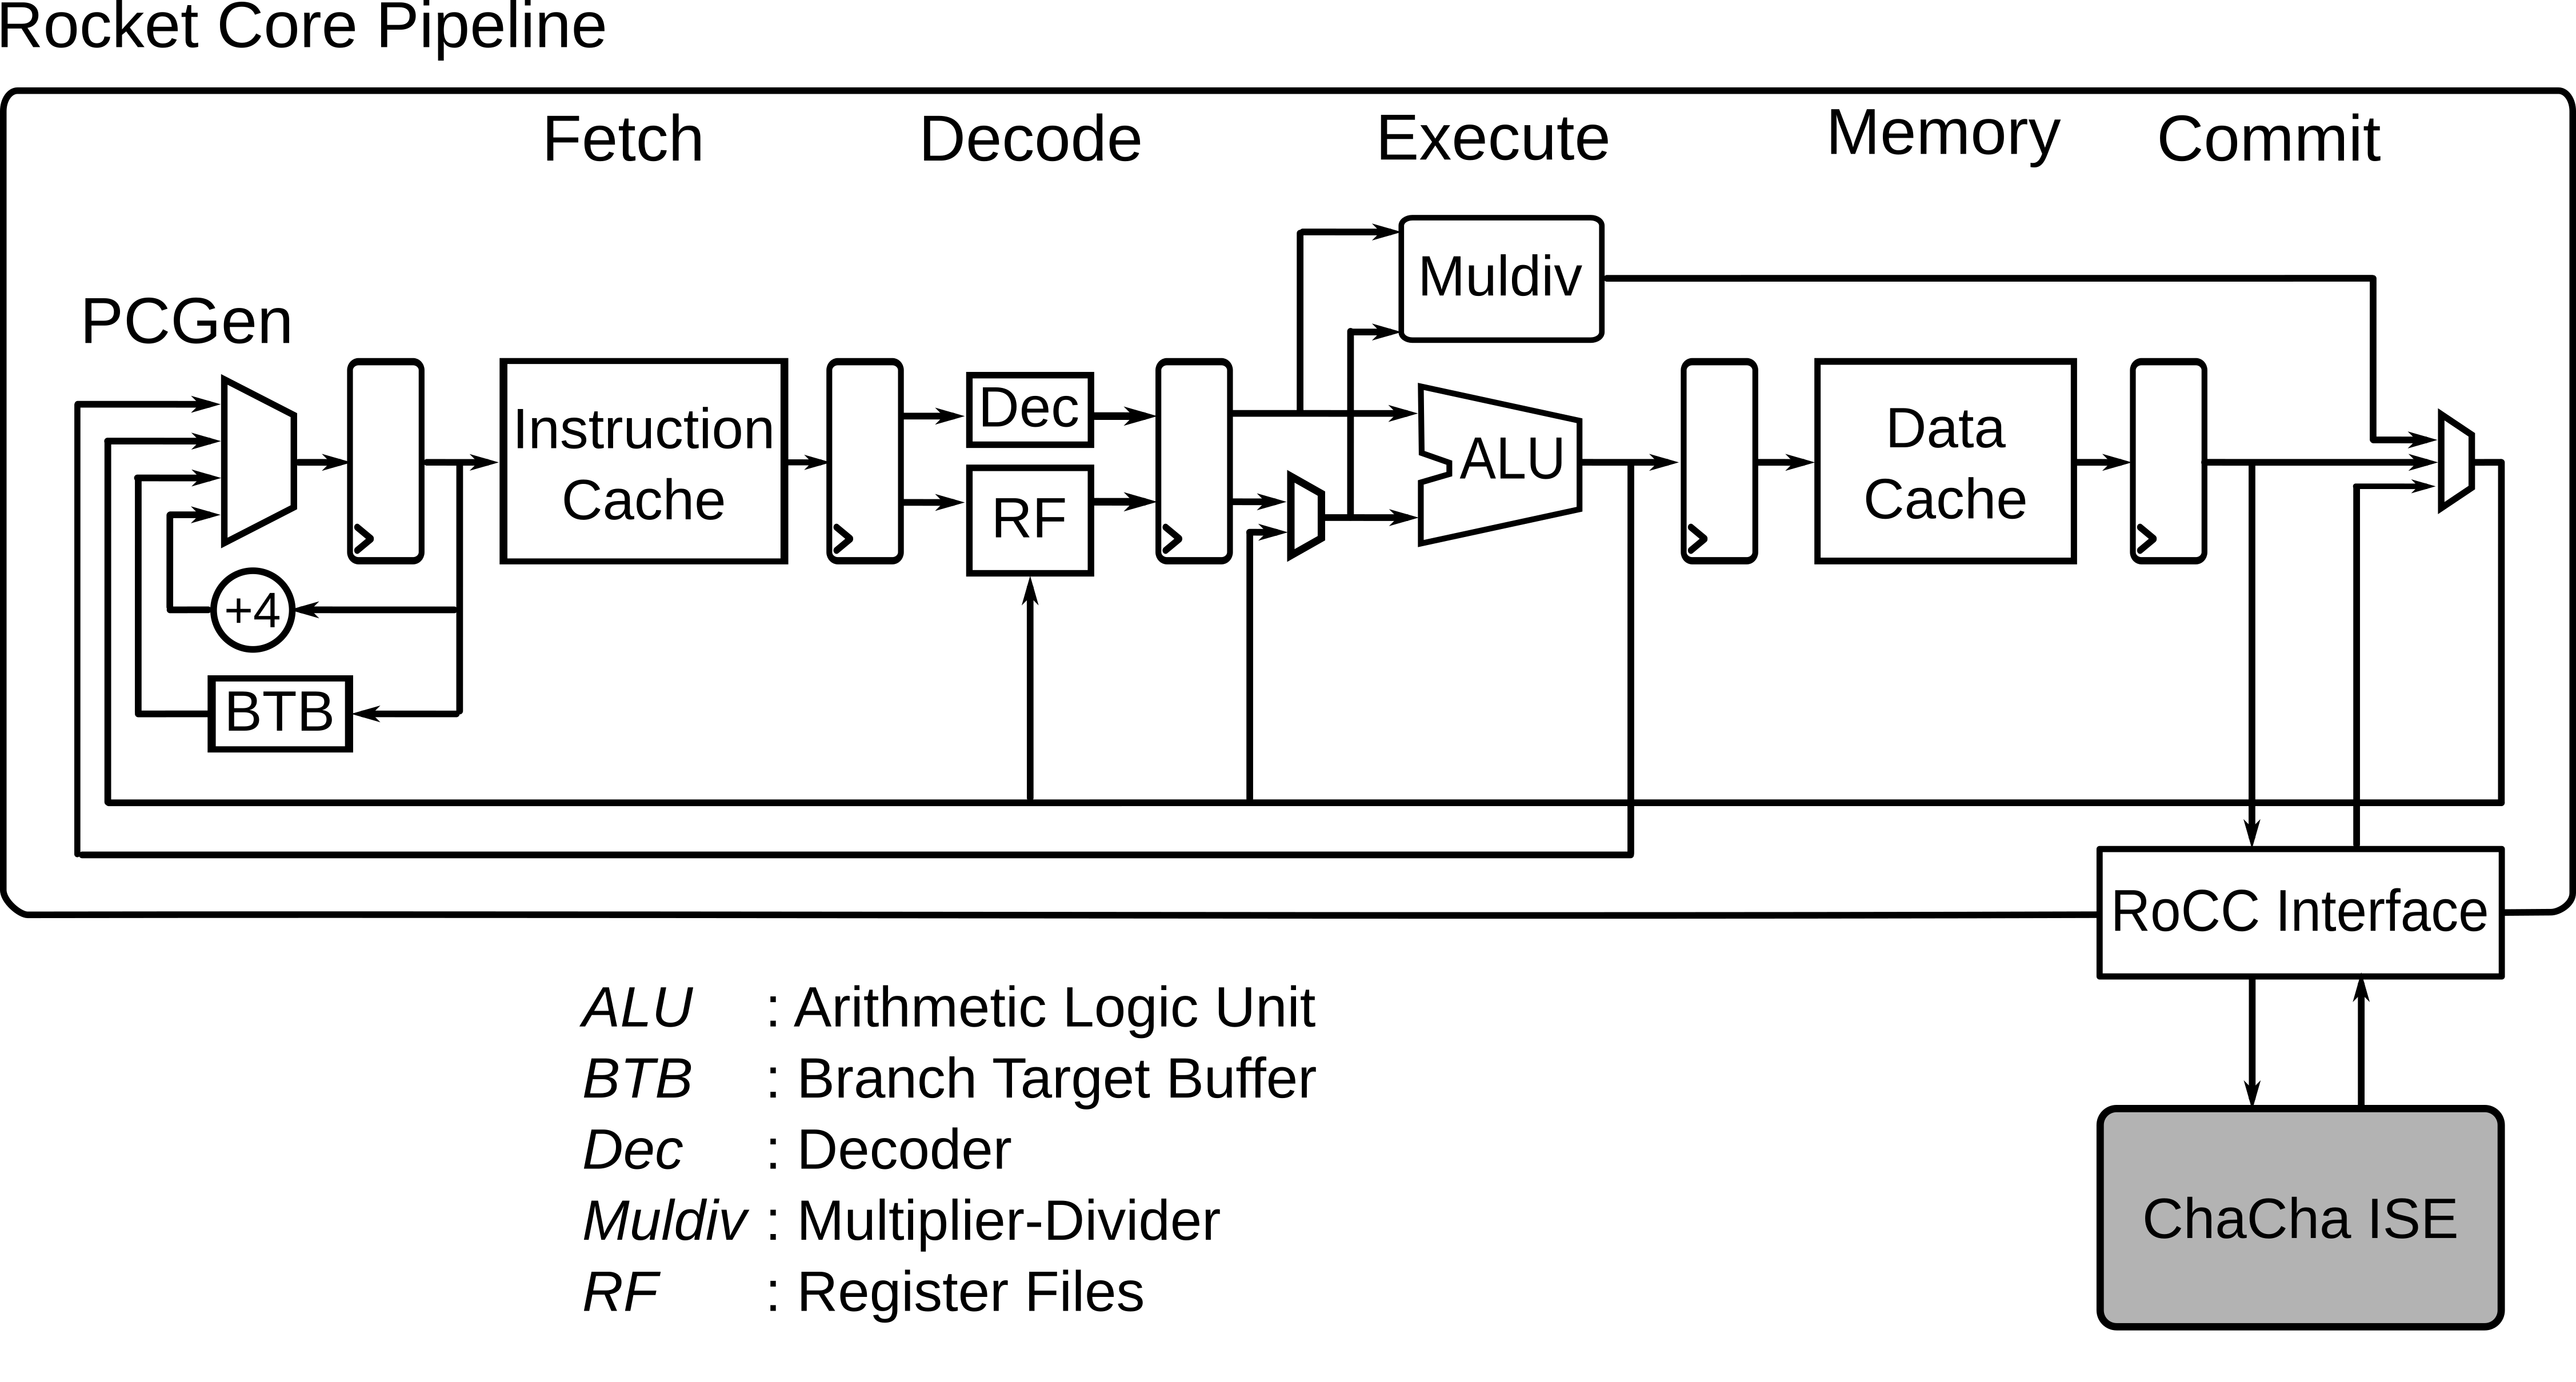
\includegraphics[scale=0.8]{figures/RocketCoreRoCC.png}
	\caption{Integrating the ChaCha ISE into the Rocket Chip}
	\label{fig:ise:RocketCoreRoCC}
\end{figure}

To evaluate the proposed ISE variants, each of the ISE variants is integrated into a 64-bit RISC-V host core. 
We opt for a well-known Rocket Chip~\cite{rocket:16} as the host core for ChaCha ISEs. 
The Rocket core is a highly configurable RISC-V core that executes instructions using a 5-stage, in-order pipeline. 
We take advantage of this to configure for a core supporting RV64IMC instruction set, i.e., the 64-bit base integer ISA~\cite[Chapter 5]{RV:ISA:I} plus standard Multiplication~\cite[Chapter 7]{RV:ISA:I} and Compressed~\cite[Chapter 16]{RV:ISA:I} extensions. It is also configured to support an instruction cache, a data cache, and a branch prediction mechanism.
To support ChaCha ISE, the Rocket Chip core has an additional configuration to enable custom instructions, for which we choose the \VERB[asm]{Custom 0} opcode \cite[Chapter 25]{RV:ISA:I}, to decode the ChaCha ISE.
The core accesses the ChaCha ISE submodule via a Rocket Custom Coprocessor (RoCC) interface~\cite[Section 4]{rocket:16}, shown in \REFFIG{fig:ise:RocketCoreRoCC}. Since the ISE variants' implementations 
comply with at most 2 sources and 1 destination operands requirement, no further structural modification is required in micro-architecture. 

\begin{table}
	\caption{Area overheads of ChaCha ISE integration compared to Rocket core and its sub-modules}
	\label{tab:res:hardcost2}
%	\begin{tabular}{lrr}
%		\toprule            
%		Algorithm        &     Size (NAND2 gates)       & Depth \\
%		\midrule
%		RV64 Rocket core               &    98150 (1.00$\times$)  &  153  \\
%		~~~~~|-- ALU                   &     3719 (0.04$\times$)  &   28  \\
%		~~~~~|-- Muldiv                &    17171 (0.17$\times$)  &   40  \\
%		~~~~~|-- Others                &    77260 (0.79$\times$)  &    -  \\
%		RV64 Rocket + ChaCha ISE &   100101 (1.02$\times$)  &  153  \\ 
    \centering
	\begin{tabular}{lrrr}
		\toprule            
		                 &     LUTs   &   FFs  &   Slices \\
		\midrule
		RV64 Rocket core  &    9865   &  3749  & 3014 (1.00$\times$)\\
		~~~~~|-- ALU      &     603   &     0  &  169 (0.06$\times$) \\
		~~~~~|-- Muldiv   &     613   &   214  &  173 (0.06$\times$)\\
		~~~~~|-- Others   &    8649   &  3535  & 2672 (0.88$\times$)\\
		RV64 Rocket + ISE &   10231   &  3749  & 3114 (1.03$\times$)\\ 
		
		\bottomrule
	\end{tabular} 
\end{table}

%Again, we use the Yosys tool to obtain the post-synthesis circuit area of the integrated system including the Rocket core and the ChaCha ISE submodule.
We implement the evaluated systems on Kintex-7 XC7K160T FPGA device employing Xilinx Vivado 2019.1 version. 
The default synthesis settings are used, with no effort invested in synthesis or post-implementation optimisation.
\REFTAB{tab:res:hardcost2} reports the area overheads of the Chacha ISE submodule in the system in comparison to the Rocket core and its submodules, e.g. Multiplier/divisor (Muldiv), ALU. 
The implementation of $V_4$ is chosen for the ChaCha ISE submodule to report in the table because it gains the best trade-off between area overhead (see \REFTAB{tab:res:hardcost1}) and software performance (see \REFTAB{tab:res:sw:perf1}). 
As can be seen, 
the ChaCha ISE causes a small increase of 3\% in the number of logic Slices of the Rocket core, and consumes no Flip-Flops (FFs). 
In fact, its overhead is considerably smaller compared to other functional submodules such as ALU, Muldiv. 
Moreover, the timing report of the implementation result shows that the ChaCha ISE does not affect the longest delay paths which reduce the maximum operating frequency of the system.



